%###
\documentclass[conference]{IEEEtran} \makeatletter \def\ps@headings{%
\def\@oddhead{\mbox{}\scriptsize\rightmark \hfil \thepage}%
\def\@evenhead{\scriptsize\thepage \hfil \leftmark\mbox{}}% \def\@oddfoot{}%
\def\@evenfoot{}} \makeatother
\pagestyle{headings}
\usepackage[utf8]{inputenc}
\usepackage{url}
\usepackage{graphicx}
\usepackage{subfigure}
\usepackage{color}
\usepackage{algorithm}
\usepackage[noend]{algpseudocode}

\algrenewcommand{\algorithmiccomment}[1]{\# \textit{#1}}

\newcommand{\noteperso}[1]{\begin{center}
\fbox{\begin{minipage}{0.9\columnwidth}#1\end{minipage}}\end{center}}
%\renewcommand{\noteperso}[1]{}

%\renewcommand{\tablename}{Table}

\begin{document}

\title{Measuring Routing Tables in the Internet}

\author{
\IEEEauthorblockN{\'Elie Rotenberg}
\IEEEauthorblockA{UPMC Univ Paris 6, LIP6\\
CNRS, ENS de Lyon\\ \url{Elie.Rotenberg@lip6.fr}}
\and
\IEEEauthorblockN{Christophe Crespelle}
\IEEEauthorblockA{Université Claude Bernard Lyon 1, DANTE/INRIA\\ LIP, CNRS, ENS
de Lyon, Université de Lyon\\ \url{Christophe.Crespelle@inria.fr}}
\and
\IEEEauthorblockN{Matthieu Latapy}
\IEEEauthorblockA{UPMC Univ Paris 6, LIP6\\
CNRS\\ \url{Matthieu.Latapy@lip6.fr}}
}

\maketitle


\begin{abstract}
The most basic function of an Internet router is to decide, for a given packet,
which of its interfaces it will use to forward it to its next hop. To do
so, routers maintain a routing table, in which they look up for a prefix of the
destination address. The routing table associates an interface of the router to
this prefix, and this interface is used to forward the packet. We explore here a
new measurement method based upon distributed UDP probing to estimate this routing table for Internet routers.
 
\end{abstract}

\section{Introduction}
\label{sec:intro}
The role of Internet routers is to forward packets locally to ensure that at the
global scope, the packets traveling through the network will reach their
destinations. The routing heuristics are diverse, but the result of
routing itself can always be seen as a collection of pairs of a packet, and an
interface of the router, which it uses to pass the packet to its gateway for its
next hop.


However, the details of how this interface is chosen are diverse, and generally
not publicly disclosed. The exact nature of the decision leading to the choice
of a particular interface for a given packet can depend on multiple factors,
including the destination address prefix, the AS of the destination, the packet
IP identifier, static configuration, random or pseudo-random load-balancing
factors, and more, implementing the routing policy of the router. In its most
general definition, a routing table of a router $r$ is a set of rules that
design which interfaces of $r$ should be used to send or forward a message
towards a given destination. It is a set of rules where each rule $D \rightarrow
I$ indicates that for any given destination $d \in D$, an interface $i \in I$
should be used by $r$ to send a message towards $d$. The sets $D$ of destination
are either included one in another or disjoint for consistency. (In practice,
each $D$ is often a set of destination addresses matching a certain binary
prefix)


The knowledge of the actual routing tables, resulting from both static and
dynamic configuration, is critical for understanding and modelling routing in
the Internet topologies. They define the local behavior of the routers
from which the global behavior of the network emerges.


We present here a measurement method that allows to estimate partially
or totally such ``routing tables''. We use a measurement primitive, UDP Ping, to
measure the interface used by a target router to route traffic back towards
a given monitor source (Section~\ref{sec:udpping}).
This primitive is used repeatedly from a large amount of distribution monitors
to gather information (Section~\ref{sec:distribudpping}). This information is then
processed into constraints on the rules of the routing table
(Section~\ref{sec:constraints}). Several assumptions may then be used to further
infer these rules, estimating more practically the possible routing table of
the target routers (Section~\ref{sec:inference}). We finally assess the
principle of this method by conducting a series of practical measurements
(Section~\ref{sec:measurement}).


\section{Measurement method}
\label{sec:measurementmethod}
\subsection{UDP Ping}
\label{sec:udpping}

UDP Ping is a measurement primitive inspired by IP aliasing techniques that we
have developped in the context of router degree
measurement~\cite{udpping2013}, which allows to discover the interfaces used
by a target router to send messages towards monitors that we control.

Let $t$ be an IP adress which we call the \emph{target}, and $r(t)$ the node
(router or end-host) to which $t$ belongs. RFCs \cite{rfc1122} and
\cite{rfc1812} state that when a monitor $m$ sends an UDP packet with
destination $t$ on an unallocated port, then $r(t)$ should answer with and ICMP
Destination Unreachable packet to $m$. An important detail is that the source of
this ICMP packet is in principle the IP address of the interface $i$ used by
$r(t)$ to send packets towards $m$.
(See \figurename~\ref{fig:ping-udp})

\begin{figure}[!h] \centering
\resizebox{.7\columnwidth}{!}{\input{figures/ping_udp.pstex_t}}
\caption{Monitor $m$ sends a UDP packet with destination address $t$ on an
unallocated port; the node $r(t)$ answers with an ICMP packet with source
address $i$, and thus $m$ discovers interface $i$ of $r(t)$.}
\label{fig:ping-udp}
\end{figure}

We have studied extensively UDP Ping in a previous work \cite{udpping2013}. We
concluded that when $r(t)$ properly implements the RFCs (which we can detect
for a given router), then it allows to reliably discover its interfaces.
A single run of UDP Ping from a monitor $m$ leads to the observation of an
interface $i$ used by $r(t)$ to route towards $m$. However, $r(t)$ may not
always use $i$ to route towards $m$. To capture all such interfaces, we use UDP
Ping repeatedly to observe all of them. The set $m(t) = \{ i_1, i_2, \ldots \}$
constructed by repeatedly probing $r(t)$ from $m$ is the set of all the
interfaces that $r(t)$ uses to route towards $m$.

\subsection{Distributed UDP Ping}
\label{sec:distribudpping}

While UDP Ping itself only provides information on the interfaces used by a
target to route towards a given monitor, it can be used distributedly to gather
complete information depending on the quality of the monitor set.
As explained in \cite{CLR10}, the distributed usage of UDP Ping
from a monitor set that is large enough and well distributed in the Internet allows to
discover all the network interfaces of Internet core routers. Instead, border
interfaces would be very hard to observe.

Depending on the configuration of the target, the topological meaning of ``well
distributed'', \emph{i.e.} ``leading to the inference of many rules'', could be
well distributed in the IPv4 adressing space, or in ASes.

Given a monitor set $M = \{ m_1, m_2, \ldots \}$, using UDP Ping from each
monitor towards a target $t$ leads to the observation of a set $M(t) = \{ (m,
m(t)) \}$, where $m$ is an IP address and $m(t)$ is the set of interfaces of
$r(t)$ used to forwards packets towards $m$.


% However, the distributed nature of the measurement, and thus the  is only
% significant if the monitor set is both large and well distributed. Indeed, \cite{udpping2013} has
% shown that colocated monitors (monitors that are located very close to each other in the
% network) lead to very similar, redundant observation. In order to achieve
% effective discovery, the monitor set should be well distributed in the network.
% Depending on the configuration of the target, this could mean to be well
% distributed in the IPv4 adressing space, or in ASes. One of the purposes of the
% current study is to help discover which characteristics of the monitor set are
% required to efficiently explore the interfaces usage of a target.

\section{Constraints obtained from measurement}
\label{sec:constraints}

The routing tables of routers have structural specificites
(Section~\ref{subsec:rules}) that allows us to use the results of the
measurement method described in Section~\ref{sec:udpping} to deduct constraints on the routing
table of a given target router (Section~\ref{subsec:constraints}).

\subsection{Structure of the rules}
\label{subsec:rules}

As presented in Section~\ref{sec:intro}, the routing table of a router $r$ is
composed of a list of rules $\{ D_k \rightarrow I_k \}$, where $D_k$ is a set of destination
addresses, and $I_k$ is the set of interfaces used by $r$ to route towards the
destinations in $D_k$.

By design, routing tables share a number of structural properties resulting from
basic optimization concerns. (1) the interface sets are minimal: each
interface in a given $I_k$ is actually used to route towards each destination in
$D_k$ (no ``unused'' interface in $D_k$). (2) two destination sets $D_k$ and
$D_{k'}$ are either included one in another, or disjoint, so that the
most-specific destination set lookup for a given destination is fast. (3)
thanks to the very high practictal efficiency of dedicated hardware, each $D_k$
is usually a \emph{prefix class}: there exist a binary prefix $p_k$ of
length $n_k$ such that $D_k$ is exactly the set of IP addresses that match
$p_k$.
We then denote $D_k = p_k/n_k$. In this form, the rules can be conveniently
represented in an actual table (See \figurename~\ref{fig:table-example}), hence
the name ``routing table''. (4) as a consequence of (2) and (3), there can not be
two rules $p.0 \rightarrow I$ and $p.1 \rightarrow I$: they would be replaced by
a single, equivalent rule $p \rightarrow I$.

\begin{figure}
\begin{center}
\begin{tabular}{| p{.15\columnwidth} | p{.4\columnwidth} | p{.3\columnwidth} |}
\hline
Rule $k$ & Destination prefix $p/n$ & Exit interface(s) $I$ \\ \hline
1 & 128.32.0.0/13 & 83.238.96.26 \\ \hline
2 & 128.40.0.0/13 & 195.114.175.54 \\ \hline
3 & 128.112.139.64/26 & 83.238.96.26 \\ \hline
4 & 128.112.139.0/26 & 83.238.96.26, 195.114.175.54 \\ \hline
5 & 128.114.63.0/26 & 83.238.96.26, 195.114.175.54 \\ \hline
\ldots & \ldots & \ldots \\ \hline
\end{tabular}
\end{center}
\caption{Example of a routing table. The router has two interfaces,
83.238.96.26 and 195.114.175.54. If the router needs to route a packet,
it choses the longest matching prefix from its table and forwards it to the
next gateway through one of the exit interfaces. Rule 1 matches a prefix of
length 13. Rules 4 and 5 show examples of multiple exit interfaces
configurations, probably implementing a form of load-balanding.}
\label{fig:table-example}
\end{figure}

\subsection{Constraints from Distributed UDP Ping}
\label{subsec:constraints}

The results from Distributed UDP Ping from a monitor set $M$ towards a router
$r(t)$ (Section~\ref{sec:measurementmethod}) can be interpreted in terms of
rules of the routing table of $r$.

Distributed UDP Ping outputs a list $M(t) = \{ (m, m(t) \}$ where each $m$ is an
IP address and $m(t)$ is the set of all the interfaces of $r(t)$ uses to route
towards $m$. This means that for any rule $D_k \rightarrow I_k$ in the routing
table of $r(t)$ such that $m \in D_k$, then each interface in $m(t)$ is
also in $I_k$, \emph{i.e.} $m(t) \subseteq I_k$.
Conversely, since \emph{all} the interfaces used by $r(t)$ to route towards $m$ are in
$m(t)$, then $I_k \subseteq m(t)$. In terms of prefixes, this means that there
must exist a prefix $p_m/n_m$ such that $m$ matches $p_m$, $p_m/n_m \rightarrow
m(t)$, but also that for each $m'$ also matching $p_m$, then $m(t) = m'(t)$.

Therefore, the constraints deducted from the observation from each monitor $m$
are:
\begin{itemize}
  \item There must exist a rule $p/n \rightarrow m(t)$ such that $m$ matches
  $p$. (\emph{Existence constraint})
  \item For each rule $p'/n' \rightarrow I$ such that $m$ matches $p'$, then $I
  = m(t)$. (\emph{Consistence constraint})
\end{itemize}

Note that the constraints deducted from the measurement largely depend on the
nature of the monitor set $M$. For exemple, let us assume that two monitors
$m_0$ and $m_1$ are such that $m_1(t) \neq m_2(t)$, and their longest common
prefix is $p$, such that $m_0$ matches $p.0$ and $m_1$ matches $p.1$. Then their
can be no rule $p/n \rightarrow I$ in the routing table of $r$ for any $I$, nor
any rule $p'/n' \rightarrow I$ where $p'$ is a prefix of $p$. The implications
of this constraint largely depends on $p$, therefore on the adresses of $m_0$
and $m_1$.

\section{Routing table inference}
\label{sec:inference}

The constraints retained from observation in ~\ref{subsec:constraints} don't
directly provide an estimate of the routing table. Many routing table are
compatible with these constraints. However, combining the constraints with
additional assumptions allows us to infer realistic rules.
We will examine three inference patterns, using different assumptions to infer
the routing table of a router.

\subsection{Most specific routing table}
\label{subsec:mostspecific}

The most simple inference pattern simply translates the \emph{Existence
constraint} from Section~\ref{subsec:constraints} into rules, using the trivial
prefix $m/32$ for each monitor $m$ : $m/32 \rightarrow m(t)$. We then merge
duplicate rules as described in Section~\ref{subsec:rules}(2). The
\emph{Consistence constraint} is trivially ensured, since each rule is either of
prefix-length 32 or resulting from a duplicate merge.

This routing table is rigorously consistent with the observation, and makes no
additional assumption at all. However, its reach is very limited, since it only
provides routing information towards destination inside our monitor set. We name
this infered table the \emph{most specific routing table}.

\subsection{Generalizing hypotheses}

At the extreme opposite of the \emph{most specific} routing table
(Section~\ref{subsec:mostspecific}), there is another routing table that is
compatible with the observation: the \emph{least specific} routing table. It
consists on the set of rules with the largest sets of destinations (or the
shortest prefixes) that are compatible with the \emph{Consistence constraint}
from Section~\ref{subsec:constraints}.
While this routing table is very general, however, it is very hard to ensure its
completedness:
one may find a destination $d$ which, if added to $M$, would produce
incompatible rules.
For example, if $M$ is a single monitor $m_1$ such that $m_1(t) = \{i_1\}$, then
the \emph{least specific} routing table consists in only one rule, $\{
\emptyset/0 \rightarrow \{i_1\}\}$ (``empty prefix routes using $i_1$''). If there
exists a host $m_2$ such that $m_2(t) \neq \{i_1\}$, then adding $m_2$ to the monitor
set makes the routing table incompatible. Note that, the larger and the better
distributed $M$ is, the harder it is to find destinations that are not
compatible with the routing table, thus the more relevant the least specific
routing table is.

The actual routing table of a router is somewhere between the most specific
(``least informative but most accurate'') and the least specific (``most
informative but least accurate'') routing table. Using well-chosen
\emph{generalizing hypotheses}, we can extend the rules infered from the
Existence constraint. Such a generalizing hypothesis consists in an assumption
on the structure of the prefixes in the ruleset. It can be elaborated by leveraging
knowledge on the networks, such as practical constraints or common
implementations. In addition to the least specific routing table
in Section~\ref{subsec:cidr}, we will discuss one such generalizing hypothesis
based on AS prefixes in Section~\ref{subsec:cidr-as}.

\subsection{CIDR prefixes generalization}
\label{subsec:cidr}

The least specific, most generalized routing table is actually a generalizing
hypothesis resulting from the \emph{CIDR} convention. For many reasons, among
which the practical size of the routing tables, the \emph{CIDR} address
allocation method \cite{rfc1518,rfc1519,rfc4632} was introduced in 1993 and is
now a both formal and practical standard. The adoption of CIDR means that
subnetworks are characterized by address prefixes. This allows for efficient
routing table compression, since the rules can be expressed in the form of
prefix-matching rules, both easy to lookup using dedicated hardware
\cite{Mcauley93fastrouting} and of small size compared the classful rules of the
early Internet. From an inference point of view, this means that each
prefix-based rule only needs one representant to be discovered. The least
specific routing table is the routing table in which the prefixes are as small
as possible while remaining compatible with the observation.
Algorithm~\ref{algo:infertable} is designed to construct this table efficiently.

\subsubsection{Inference algorithm}

\begin{algorithm}
\caption{CIDR table inference}
\label{algo:infertable}
\begin{algorithmic}[0]
\Function{Split}{$I$, $p$, $a$, $b$} \Comment{Returns a pivot to split the
subset $I[a, b]$ with a $1$ increment in prefix length}
	\State $p' \gets$ $p$.append($"1"$) 
	\State \textbf{return} binary search $I[a, b]$ for the first address starting
	with $p'$
\EndFunction
\Function{AllSame}{$I$, $a$, $b$} \Comment{Checks whether all the values in
the subset $I[a, b]$ are identical}
	\ForAll{$k \in [$\textsc{next}($a$)$.. b]$}
		\If{$\textsc{H}(I[k]) \neq \textsc{H}(I[a])$} \Comment{Hashes of the values
		are used for constant-time comparisons}
		\State \textbf{return} \textsc{False}
		\EndIf
	\EndFor
	\State \textbf{return} \textsc{True}
\EndFunction
\Function{InferSubTable}{$I$, $p$, $a$, $b$}
	\If{\Call{AllSame}{$I$, $a$, $b$}}
		\State \textbf{return} $\{"p \rightarrow I[a]"\}$
		\Comment{Adds a rule to the ruleset}
	\Else	
		\State $a', b', c' \gets a, $ \Call{Split}{$I$, $p$, $a$, $b$}$, b$
		\State $R_0 \gets$ \Call{InferSubTable}{$I$, $p$.append($"0"$),
		$a'$, prev($b'$)}
		\State $R_1 \gets$ \Call{InferSubTable}{$I$, $p$.append($"1"$),
		$b'$, $c'$} \State \textbf{return}  $R_0 \cup R_1$				
	\EndIf
\EndFunction
\Function{InferTable}{$I$}
	\State Sort $I$ by IP address in binary form \Comment{Exposes \textsc{prev},
	\textsc{next}, \textsc{bsearch}, \textsc{first} and \textsc{last} for the keys
	of $I$.}
	\State Hash the values in $I$ \Comment{Exposes H for
	the values in $I$}
	\State \textbf{return}
	\Call{InferSubTable}{$I$, $""$, $\textsc{first}(I)$, $\textsc{last}(I)$}
	\Comment{Initial call with empty prefix}
\EndFunction
\end{algorithmic}
\end{algorithm}

$I$ is an associative map indexed with the monitor adresses that contains the
set of observed interfaces for a given target when responding to each monitor,
\emph{i.e.} $I[m] = m(t)$, and $I[a, b]$ designates the list of $I[k]$ for $a
\leq k \leq b$. The algorithm first sorts $I$ by keys so that it can perform a
fast binary search of prefixes cuts. The main recursive function returns, for a
given binary prefix $p$ and a contiguous subset of $I$ (described by its
boundary keys $a$ and $b$), the set of rules required to be consistent with
the data containing the least number of rules with the shortest (most general)
prefixes. To do so, it recursively calls itself with increasingly long prefixes,
stopping when the subset is either empty or all its elements observe the same
interface set (indicating that they can be grouped under a single rule). If at
least two elements of the subset require different rules, then the prefix length
is increased to further differentiate the subsets.

\subsubsection{Proof and speed of the algorithm}

Algorithm~\ref{algo:infertable} consists in one entry routine and three
subroutines.

The subroutine \textsc{Split}($I$, $p$, $a$, $b$) takes 4 arguments:
$I$ is a lexically key-sorted dictionary, containing key-values pairs. Each key
is a monitor identifier (its IP address) and each value is the set of the
interfaces observed by this monitor for the given target. $p$ is a binary
prefix, represented by a byte row. $a$ and $b$ are monitor addresses. It is
assumed that the subset $[a,b]$ of keys lexically comprised between $a$ and $b$
share a common prefix $p$.
\textsc{Split} returns the first (in lexical order) monitor address $x$ such
that all the keys $x_0 < x$ match the prefix $p.0$ and all the keys $x_1 \geq x$
match the prefix $p.1$.
Since $I$ is lexically sorted, then $[a,b]$ is lexically sorted too and a binary
search allows to find $x$ in $O(lg(|[a,b]|))$.

The subroutine \textsc{AllSame}($I$, $a$, $b$) takes 3 arguments defining a
subdictionary $I[a,b]$ of sets of observed interfaces indexed by observing
monitor. \textsc{AllSame} tests whether all the elements $I[x]$ for $x \in [a,
b]$ are equal. This is achieved by comparing each $I[x]$ for $a < x \leq b$ to
$I[a]$. If at least one element doesn't match, the routine returns
\textsc{False}. Otherwise, it returns \textsc{True}. By pre-hashing the values
of each $I[x]$, the equality test is performed in $O(1)$, and the full execution
of the routine completes in $O(|[a,b]|)$.

The core subroutine \textsc{InferSubTable}($I$, $p$, $a$, $b$) takes 4
arguments, under the same restrictions as the arguments of \textsc{Split}. It
returns a list $R$ of rules in the form $p_k \rightarrow I_k$ such
that:
\begin{itemize}
  \item $R$ is consistent with the observation, \emph{i.e} if $x$ matches $p_k$
  then $I[x] = I_k$.
  \item $R$ is minimum, \emph{i.e.} there exists no ruleset $R'$ such that $|R'|
  < |R|$ and $R'$ is consistent with the observation.
\end{itemize}
This can be proven by recurrence on the value of $n = P_{max} - |p|$ where
$P_{max} = 32$ is the maximum prefix length.

If $n = 0$, then $p$ is a full-length prefix, actually matching exactly one
address, $a = b$. Then $L = \{p=a \rightarrow I[a] = I[b]\}$ is the minimal
solution.

If $n > 0$, then there are two cases.
\begin{itemize}
\item All the elements in $I[a,b]$ are equal, in which case $L = \{p \rightarrow
I[a] = I[b] = I[x]\}$ for any $x \in [a,b]$ is the minimal consistent solution.
\item There are at least two elements in $I[a,b]$ that are not equal, say $x$
and $y$. $x$ and $y$ have atleast one different bit, proving that $p$ is not
specific enough. $p$ is further specified by appending one bit to the pattern,
either 0 or 1, using the least-specific split computed by \textsc{Split} and
calling recursively calling the subroutine with a prefix-length of $|p|+1$. By
recurrence, the two sub-solutions are optimal, and therefore the union of the
two solutions are also optimal, since there exist no solution with a
prefix-length of $|p|$.
\end{itemize}
The subroutine internal calculations are: the call to the subroutine
\textsc{AllSame}, executing in $O(|[a,b]|)$, the call to the subroutine
\textsc{Split}, executing in $O(lg(|[a,b]|))$, and finally the recursive calls.
An amortized analysis shows that for each prefix length $l' \leq |p|$, each
element $I[x]$ is only looped trough once, therefore bounding the complexity to
$O(|[a,b]|*(P_{max} - |p|))$ where $P_{max}$ is the maximum prefix length (32).

The main routine \textsc{InferTable}($I$) takes only one parameter representing
the observed data. It returns the minimum CIDR ruleset consistent with the
observation.
It firsts builds the required representation to fit the assumptions above, in
particular that $I$ is a sorted dictionary allowing for efficient binary
searches and a proper chaining allowing the usage of \textsc{next} and
\textsc{prev} on the keys of $I$. The values of $I$ are also hashed to expose a
constant-time equality test through the memoized \textsc{h} hash function.
It then calls the \textsc{InferSubTable} subroutine with the initialization
parameters: $a$ is the first key of $I$, $b$ is the last key of $I$, and the
prefix is initially empty, satisfying the required constraints.
This main entry routine performs time-consuming pre-processing. The sorting of
the keys of $I$ is $O(|M| \times lg(|M|))$ where $M$ is the number of monitors,
\emph{i.e.} the number of keys in $I$. The hashing can also be achievement in
$O(|M|)$ since the size of the hashed sets is bounded and low (no more than a
few dozens elements in the worst cases) allowing for a very efficient binary
hashing, regardless of the specific implementation of the hashing function -
any efficient generic binary hashing function will work. Last but not least, the
execution of the unique call to \textsc{InferSubTable} has a time complexity of
$O(|M|*P_{max})$. The speed of the algorithm has a total complexity of $O(|M|
\times lg(|M|))$, but has significant hidden constants, in particular for the
non-dominant terms of the complexity formula ($P_{max} = 32$ and hash function
calculations hidden constants).


\subsection{AS prefixes generalization}
\label{subsec:cidr-as}

The above method is the most generalizing, least specific hypothesis that is
consistent with the observation and in which destination classes $D_k$ match
destination prefixes. However, this assumption doesn't seem realistic, since it
can infer very short prefixes (\emph{i.e.} very general rules) based on the
sparse nature of the monitor set. To avoid too general assumption, we restrict
the selected prefixes to the prefixes advertised by ASes.

% \begin{algorithm}
% \caption{AS prefix inference}
% \label{algo:infertable-asprefix}
% \begin{algorithmic}[0]
% \State \textsc{AllSameMemo} $\gets$ \textsc{memoize(AllSame)}
% \Comment{\textsc{AllSame} is memoized to avoid redundant calculations}
% \Statex
% \Function{InferSubTableAS}{$T$, $I$, $p$, $a$, $b$}
% 	\If{\Call{AllSameMemo}{$I$, $a$, $b$} \textbf{and} ($p \in T$ \textbf{or}
% 	$|p| = 32$)} \State \textbf{return} $\{"p \rightarrow I[a]"\}$
% 		\Comment{Adds a rule to the ruleset}
% 	\Else	
% 		\State $a', b', c' \gets a, $ \Call{Split}{$I$, $p$, $a$, $b$}$, b$
% 		\State $R_0 \gets$ \Call{InferSubTableAS}{$T$, $I$, $p$.append($"0"$),
% 		$a'$, prev($b'$)}
% 		\State $R_1 \gets$ \Call{InferSubTableAS}{$T$, $I$, $p$.append($"1"$),
% 		$b'$, $c'$} \State \textbf{return}  $R_0 \cup R_1$				
% 	\EndIf
% \Statex
% \Function{InferTableAS}{$I$}
% 	\State Create a binary search tree of AS prefixes $T$ \Comment{Exposes the
% 	$\in T$ test}
% 	\State Sort $I$ by IP address in binary form \Comment{Exposes
% 	\textsc{prev}, \textsc{next}, \textsc{bsearch}, \textsc{first} and \textsc{last} for the keys
% 	of $I$.}
% 	\State Hash the values of each element of $I$ \Comment{Exposes h for
% 	the elements of $I$}
% 	\State \textbf{return} \Call{InferSubTableAS}{$T$, $I$, $""$,
% 	$\textsc{first}(I)$, $\textsc{last}(I)$}
% 	\Comment{Initial call with empty prefix}
% \EndFunction
% \EndFunction
% 
% \end{algorithmic}
% \end{algorithm}


To do so, we use an algorithm very close to Algorithm~\ref{algo:infertable}. To
account for the restriction to AS prefixes, instead of stopping the recursion
whenever a subset of monitors observe the same interface set, we continue until
the prefix is a prefix claimed by an AS, or the monitor set only has one element
(prefix length is 32), to ensure that each target is in the output table.
This can be done efficiently by looking up the prefix in a binary search tree,
based upon an official prefix registry, such as Routeviews~\cite{routeviews}.


% \subsection{Generalizing by AS}
% 
% RFCs\cite{} and vendor practices suggest that the usage of prefixes in the
% routing table is actually more an efficency of implementation constraint
% (notably due its very efficient hardware implementation using TCAM\cite{}) than
% a theoeritcal one.
% This means that routing policies and router configuration are applied at the
% AS-level semantics, and then only expanded into prefix-based syntactic rules.
% Under this assumption, if there is a prefix rule $\{r = (C(p), I)\}$, where $p$
% is one of the prefixes of a given AS, then for each prefix $p'$ also belonging
% to AS, there must be a rule $\{r' = C'(p'), I)\}$ that matches the prefix $p'$
% with the same set of interfaces $I$.


\section{Measurement}
\label{sec:measurement}

To assess the feasibility and the relevance of our approach, we have conducted a
practical measurement of Distributed UDP Ping and then performed the routing
table informance method described above.

\subsection{Repeated Distributed UDP Ping}

The repeated Distributed UDP Ping was realized from the PlanetLab platform,
consisting of 548 monitors distributed among 193 ASes. 2276 targets were chosen
among routers responding to UDP Ping probes from a previous experiment
\cite{udpping2013}.
The measure consisted in 30 repeated Distributed UDP Ping measurement towards
each target spanning over about 10 minutes.

We combined the output of the repeated measurements for each target, and
for each target, we compute its table using the methods desbribed earlier: the
most specific table, the CIDR prefixes tables, and the AS prefixes tables.

\subsection{Impact of the inference method}

\begin{figure}[!h] \centering
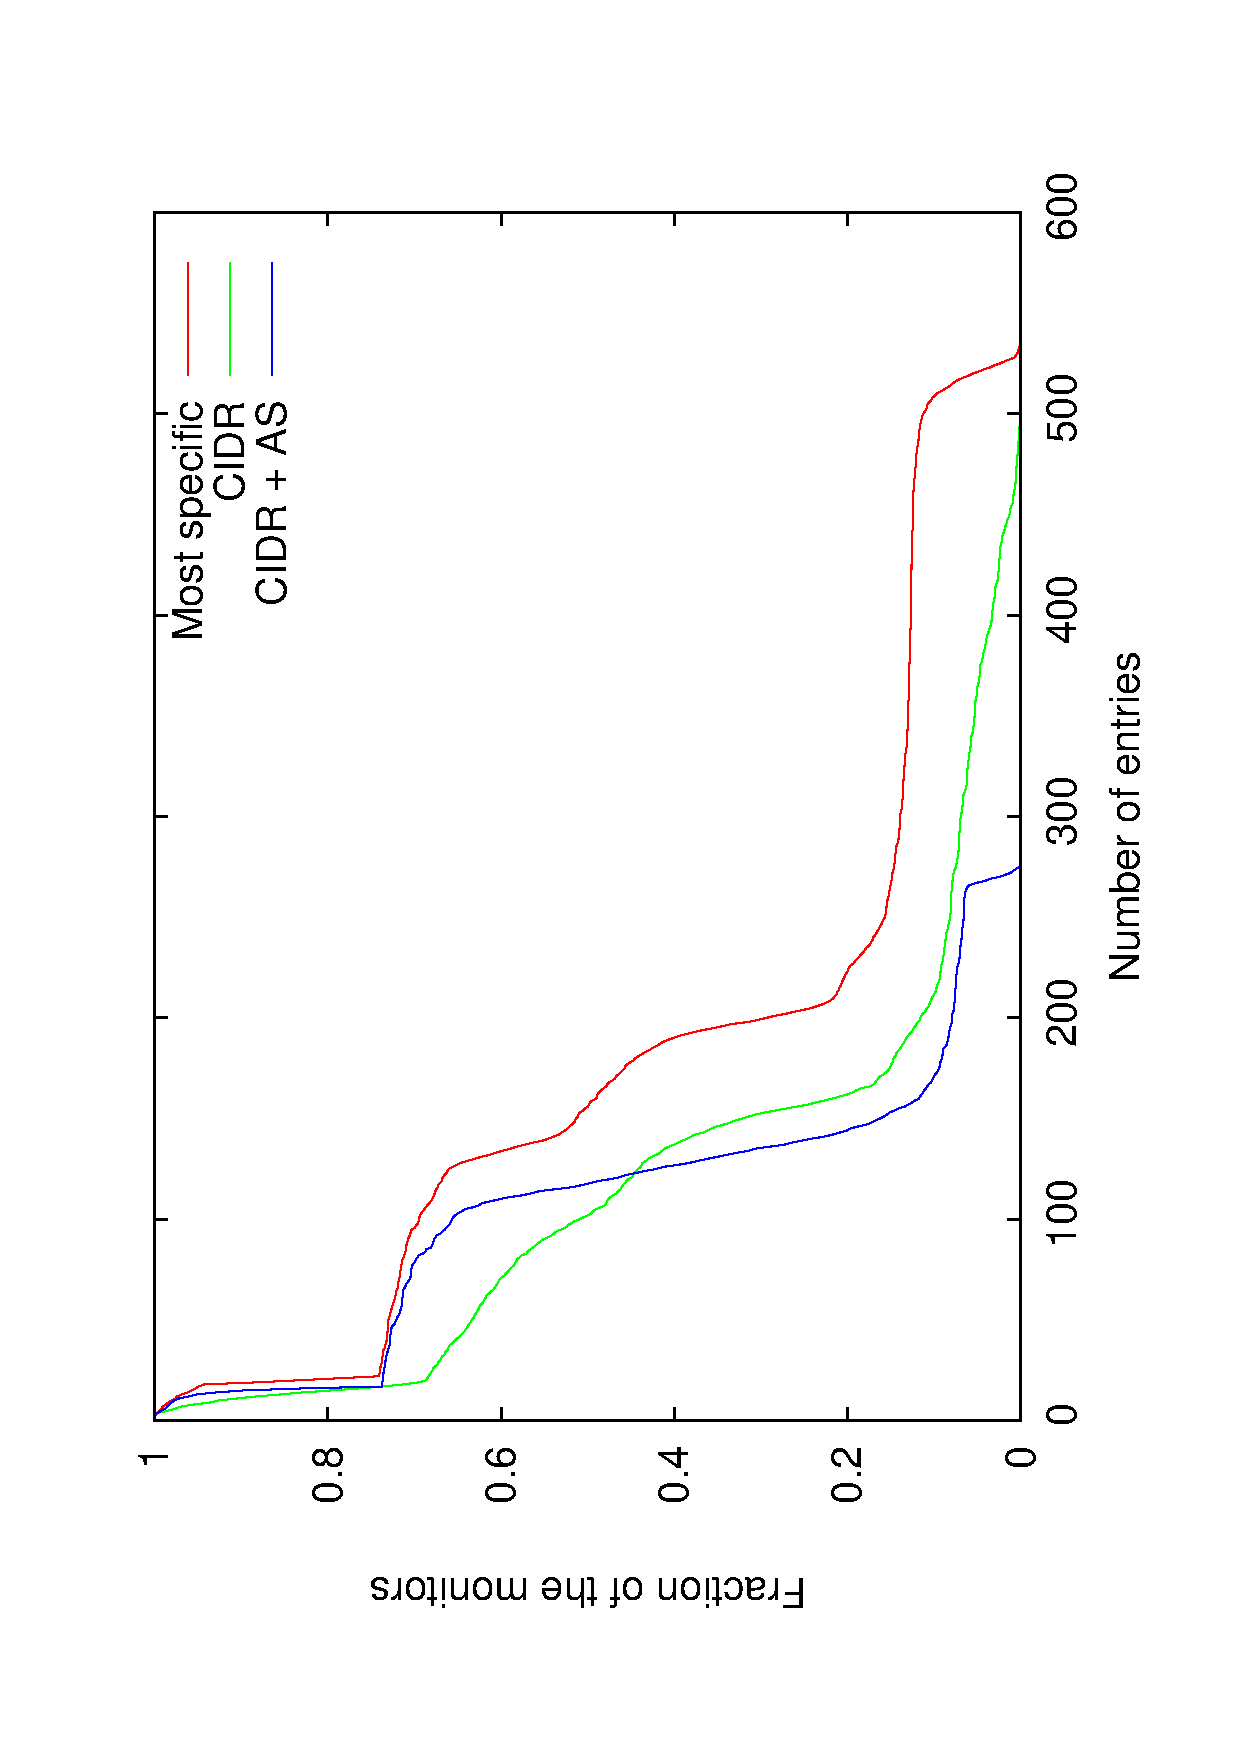
\includegraphics[angle=-90,width=.9\columnwidth]{figures/inference-refinement}
\caption{Inverse cumulative distribution of the number of entries using three
refinement methods: most specific, CIDR prefixes, and AS prefixes.}
\label{fig:inference-refinement}
\end{figure} 

After processing the observation from Distributed UDP Ping into Existence and
Consistence constraints, we used the three inference patterns describes in
Section~\ref{sec:inference} to compute estimates of the routing tables for the
target routers. For each inference pattern and for each target, we obtain a list
of rules consistent with the constraints, composed of pairs of a prefix and a
list of interfaces used to respond to monitors matching these prefixes.

We then computed the number of rules obtained for each target with the three
inference methods (See \figurename~\ref{fig:inference-refinement}). Intuitively,
for a given observation, less rules means more efficient routing table, since
the CPU and memory required to perform the routing depend on the number of rules
in the table.

The most specific routing tables have a higher number of entries,
since there is one entry per monitor which are able to observe each
target. Using AS-advertised prefixes requires less rules in the worst cases
(when the most high number of rules is required) but using the shortest CIDR
prefixes performs best for simpler tables. This suggests that in practice,
either of the two methods may be used, or mixed, to provide the most efficient
results.

\subsection{Impact of the number of monitors}

\begin{figure}[!h] \centering
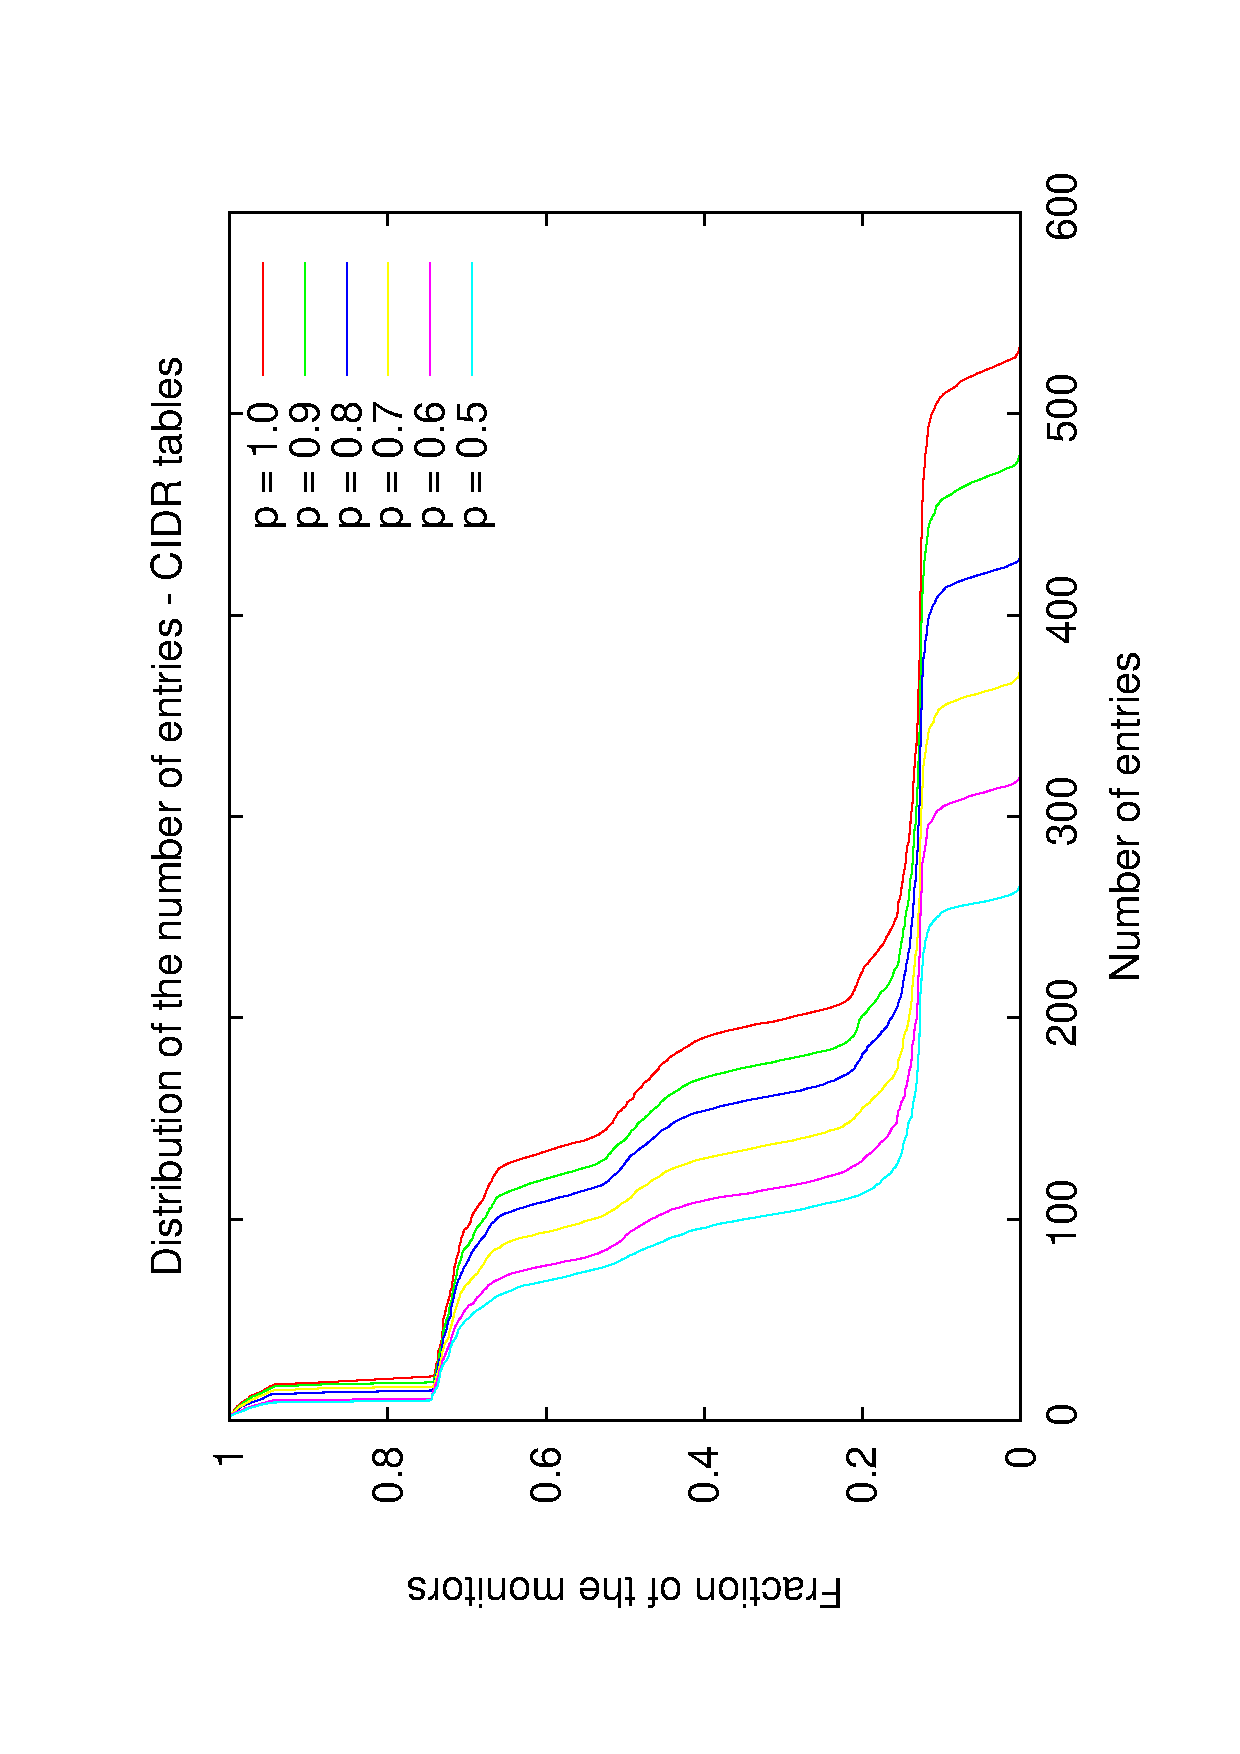
\includegraphics[angle=-90,width=.9\columnwidth]{figures/most-specific}
\caption{Inverse cumulative distribution of the number of entries in the most
specific table for several monitors subset sizes.}
\label{fig:most-specific}
\end{figure}

\begin{figure}[!h] \centering
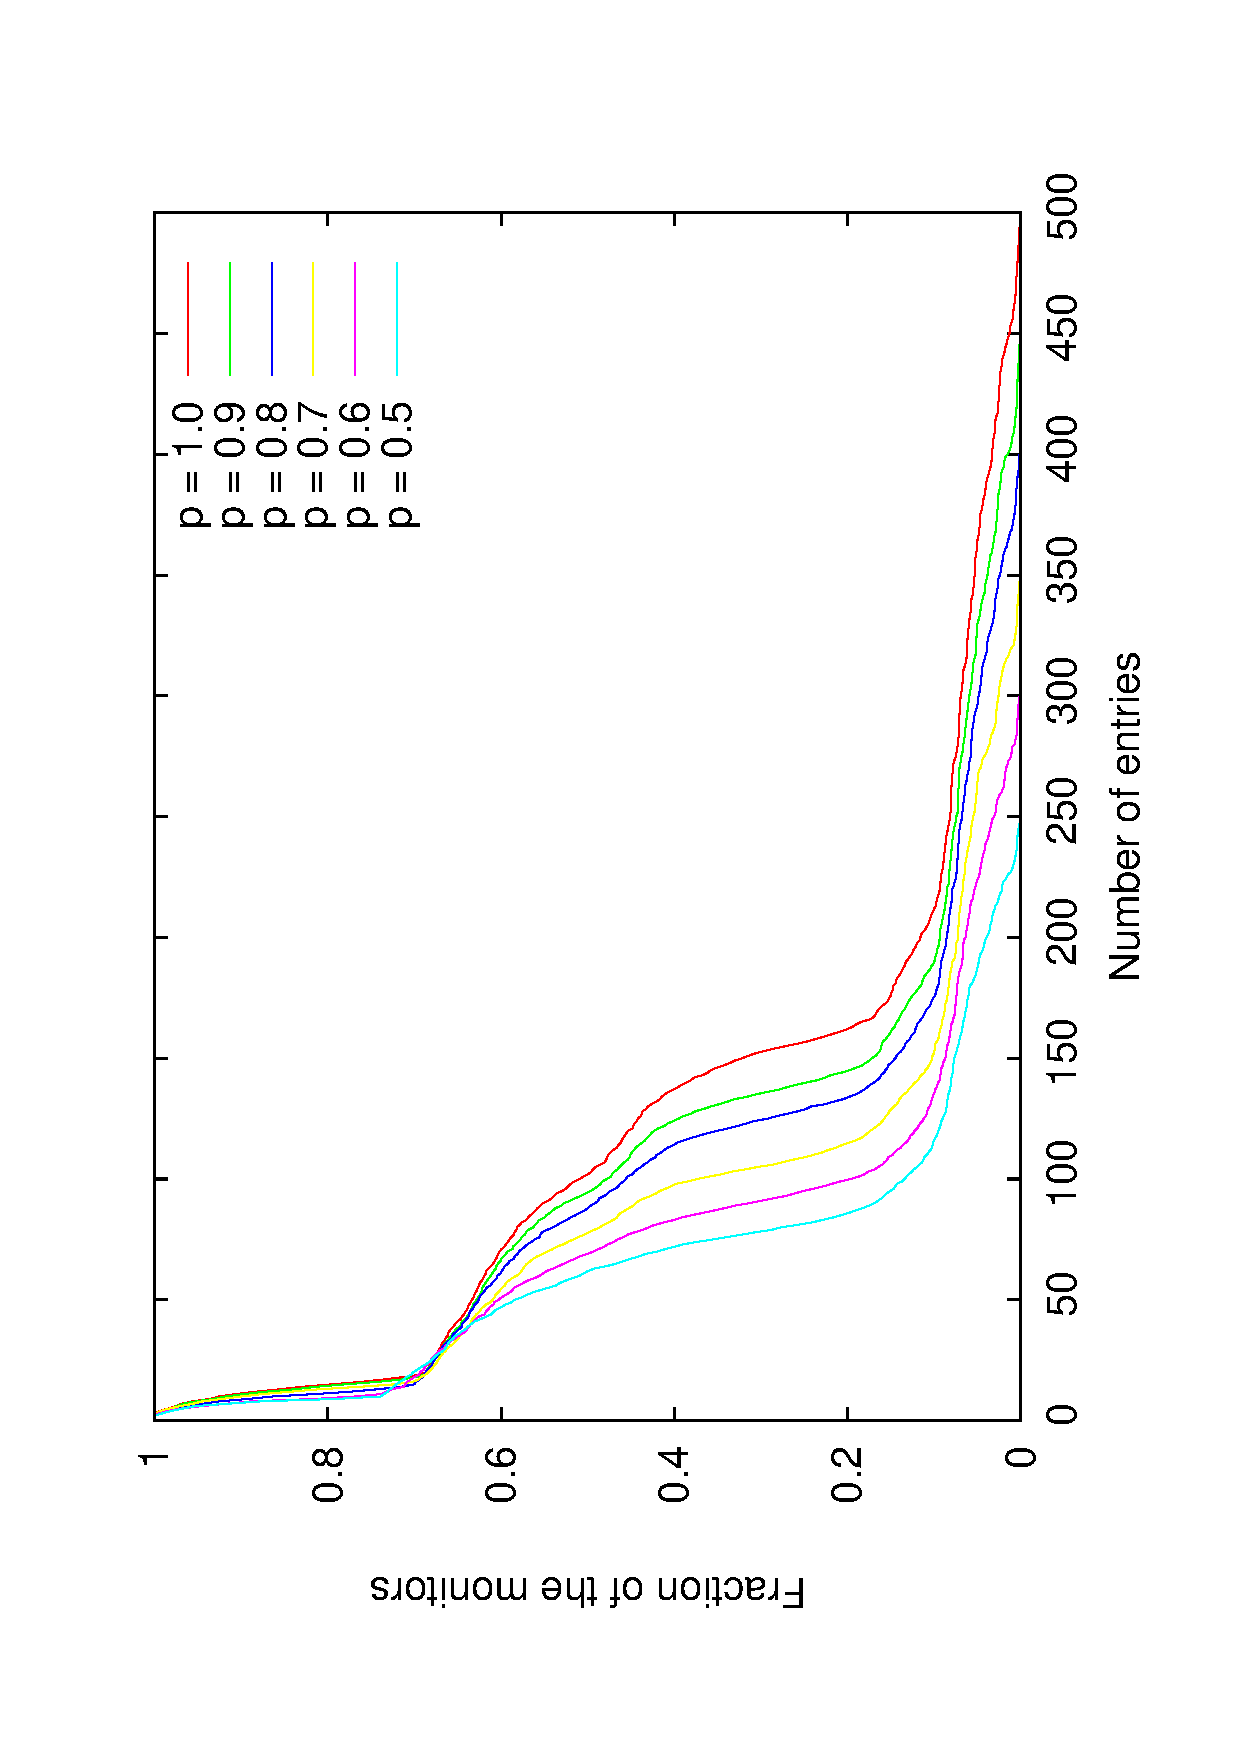
\includegraphics[angle=-90,width=.9\columnwidth]{figures/cidr}
\caption{Inverse cumulative distribution of the number of entries in the
CIDR prefixes table for several monitors subset sizes.}
\label{fig:cidr}
\end{figure}

\begin{figure}[!h] \centering
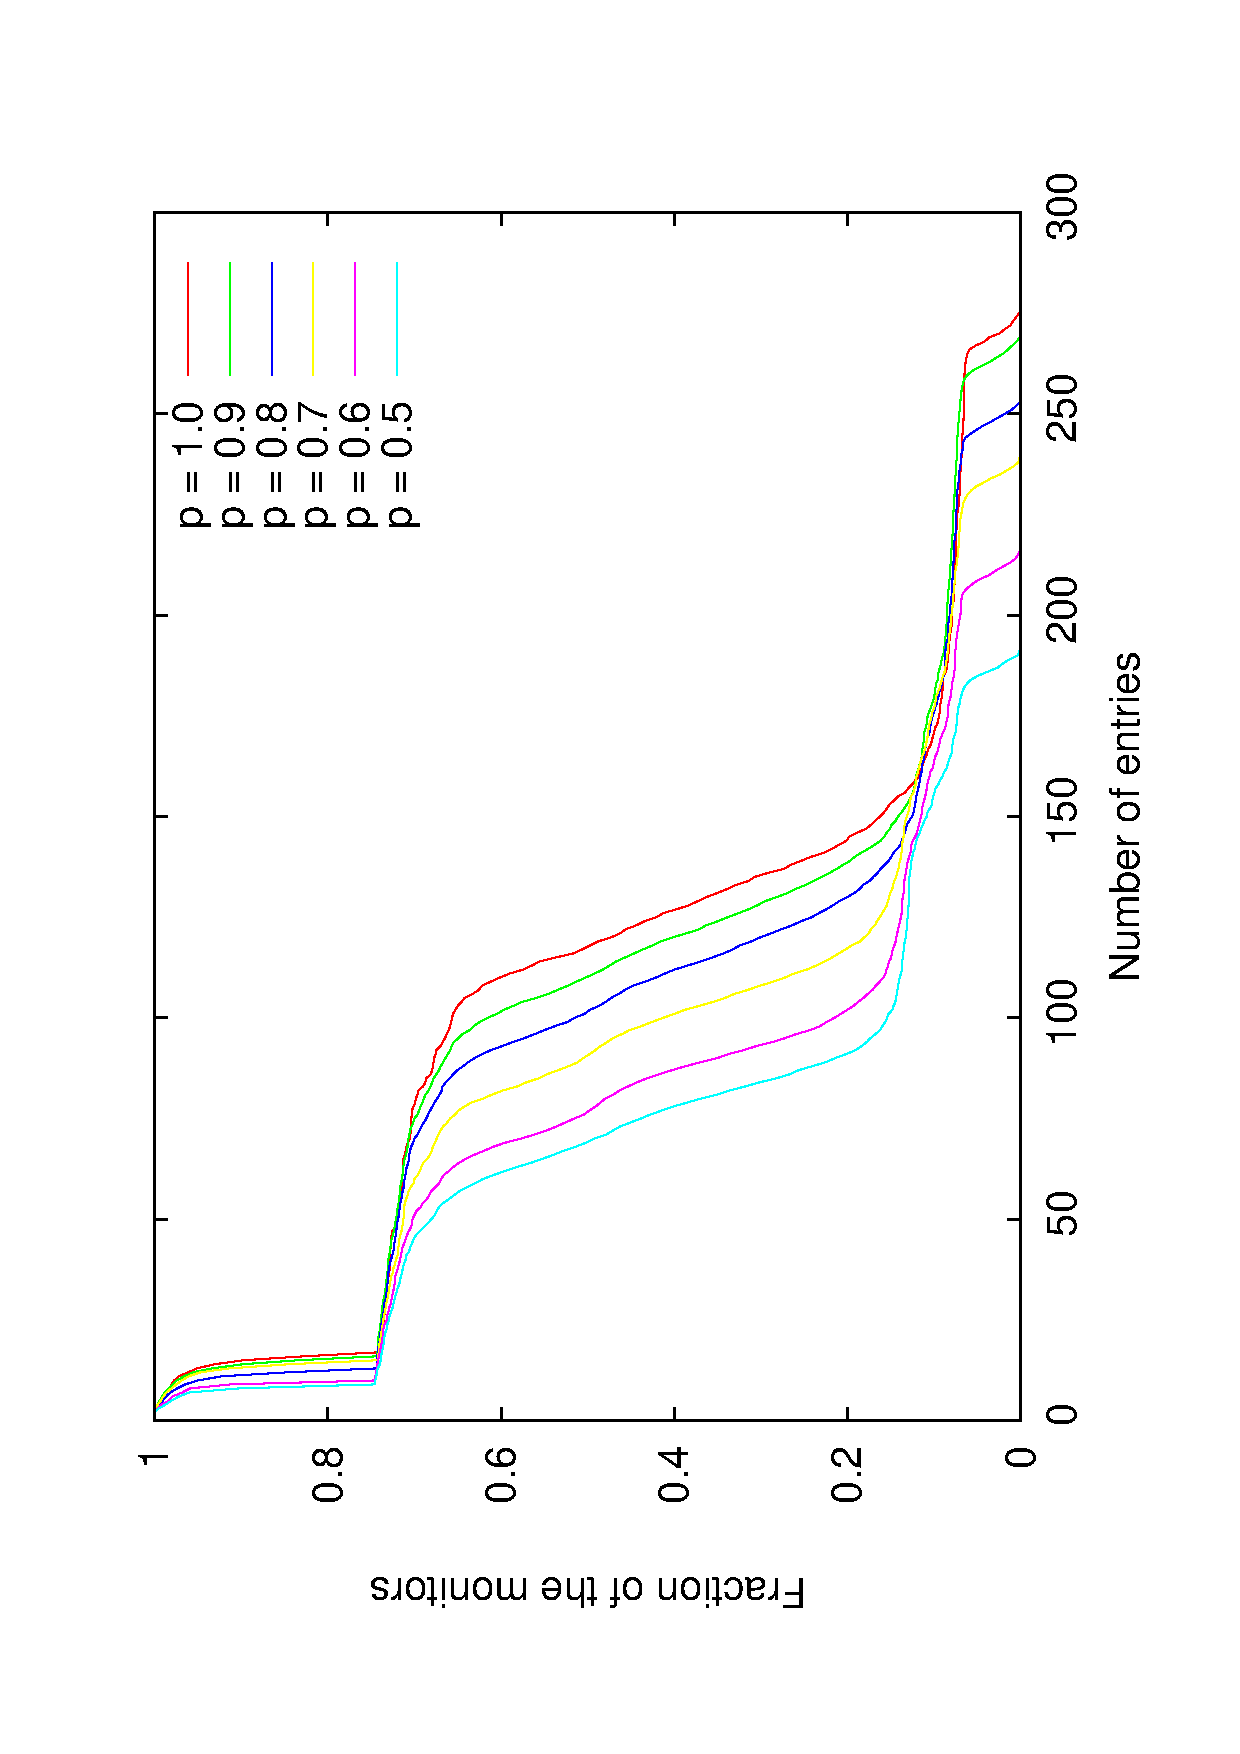
\includegraphics[angle=-90,width=.9\columnwidth]{figures/cidr-as}
\caption{Inverse cumulative distribution of the number of entries in the
AS prefixes table for several monitors subset sizes.}
\label{fig:cidr-as}
\end{figure}

We have suggested in Sections ~\ref{sec:measurementmethod} and
~\ref{sec:constraints} that the nature of the monitor set can widely affect the
nature of the observation and of the constraints. To assess the extend of this
phenomenon, we have emulated different monitor sizes by filtering the data to
only keep the results from random subsets (of given size, lower than the
maximum number of available monitors) of our complete monitor set, and comparing
the results. (See
\figurename~\ref{fig:most-specific}, \ref{fig:cidr}, \ref{fig:cidr-as})

We observe that the amplitude of the distribution depends a lot on the number of
monitors, suggesting that even if colocation is captured by the CIDR prefixes
based methods, the monitor set has not reached a steady size and could be
improved. However, the shape of the distribution remains consistent with the
monitor size, suggesting that adding monitors may give more precise, but not
completely different results.

\section{Related work}

\label{sec:relatedwork}

The physical and IP-level internet topologies are extensively studied since the
seminal papers of Pansiot {\em et al.}~\cite{280555} and Faloutsos {\em et
al.}~\cite{DBLP:conf/sigcomm/FaloutsosFF99}. The most classical approach
consists in building maps from traceroute-like measurements. However, several
studies have shown that obtained maps are intrinsically
biased~\cite{DBLP:conf/infocom/LakhinaBCX03,DBLP:journals/jacm/AchlioptasCKM09,willinger},
and even that traceroute outputs are
unreliable~\cite{paristraceroute,pansiot2012,roughan201110}.
The hope that increasing the size and quality of maps would overcome these
issues has led to much effort, but the situation remains far from
satisfactory~\cite{willinger,DBLP:conf/imw/BarfordBBC01,DBLP:conf/infocom/LatapyM08}.

Conducting precise measurements of random nodes to obtain a
reliable estimate of their behaviour was first suggested
in~\cite{DBLP:conf/infocom/LakhinaBCX03}. We explored the possibility to do so
at IP level in~\cite{CLR10} but we only partly succeeded and we conducted
thorought simulations in~\cite{CT01}.

Our work is also closely related to alias resolution (which plays a key role in
the building of maps): while we seek all (unknown) interfaces of a given router
identified by one of its interfaces, alias resolution aims at identifying in a
given set of interfaces the ones that belong to a same
router~\cite{alias-bias,keys2010internet}.
Probes similar to ours are used in this context, in particular by the
\emph{iffinder} tool~\cite{iffinder}, as well as other techniques. Our use of
such probes was clearly inspired by these works.

Finally, important efforts are devoted to the deployment of large and
distributed measurements infrastructures, which are crucial for this field of
research~\cite{caida,dimes,iplane,planetlab,ripeatlas}. Some of them distribute
monitoring capabilities at a huge scale (typically onto thousands of end-hosts)
and so are particularily promising for us \cite{ripeatlas,dimes}.

\section{Conclusion}
\label{sec:conclusion}

In this work, we have exposed the principle of using  a
distributed UDP Ping measurement to gain insight on the routing tables of the
measured targets. However, the relevance of the estimate relies highly on the
quality of the monitor set, since the inference methods only allows to
generalize rules in adress scopes (subnetworks) in which there are monitor from
the monitor set.

Besides the improvement of the monitor set, several factors could be utilized to
further infer the rules: implementation details of the routing algorithms
(namely BGP and OSPF) at the subnetwork, area and AS level, default routes, and
the usage of looking glasses. The repetition over time of this measurement and
inference method may be used to track the routing dynamics of a given target, in
particular after a BGP update.

\medskip
\noindent
{\bf Acknowledgements.}
This work is partly supported by the European Commission FP7 EULER project (grant 258307), Future Internet Research and Experimentation (FIRE), and by the DynGraph grant ANR-10-JCJC-0202 from the Agence Nationale de la Recherche.

\bibliographystyle{IEEEtran}
\bibliography{IEEEabrv,biblio}

\end{document}
%###